\chapter{Unterscheidung von Reactive Systems und Reactive Programming}\label{abgrenzung}
Im Zusammenhang mit Reactive Programming treten weitere Begriffe auf, die auch das Schlüsselwort \textit{reactive} in ihrer Bezeichnung tragen. Die \textit{Reactive Systems} sowie das \textit{Fuctional Reactive Programming}. In diesem Kapitel wird eine Differenzierung dieser Begriffe von Reactive Programming durchgeführt. Ebenso soll dadurch eine Einordnung von Reactive Programming in den Kontext der Softwareentwicklung vereinfacht werden.
\section{Differenzierung zwischen Reactive Proramming und Reactive Systems}
Bislang wurde von einem reinen Vorgehen für eine passende Implementierung gesprochen. Wie jedoch wirkt es sich aus, wenn eine komplette Anwendung reaktiv reagieren soll? Wie verhält es sich weiter wenn mehrere Teile reaktiv funktionieren und kommunizieren sollen? Der grundlegende Gedanke reaktiver Systeme wurde schon im Jahre 1985 in einem Paper von D. Harel und A. Pnueli beschrieben \cite{Harel.1985}. Zur heutigen Zeit jedoch bezieht man sich bei Richtlinien zur Gestaltung reaktiver Systeme eher auf das Reactive Manifesto \cite{Boner.2014}. Laut Jonas Bonér und den vielen Unterstützern sind vier Bestandteile essentiell, damit eine Anwendung die Anforderung erfüllt um als reaktiv zu gelten. Die Ansicht des Manifests stützt sich auf einen Architektur- beziehungsweise Designstil und soll als Grundlage zur Entwicklung reaktiver Systeme dienen. Die folgenden Erklärungen sind dem Manifest entnommen und sollen einen Verständnis zu den vier Eigenschaften bieten wie sie auch in Abbildung \ref{pic:manifest4} aufgezeigt werden. \newpage Wie in diesem beschrieben sind Reaktive Systeme:
\begin{figure}[hbt]
	\centering
	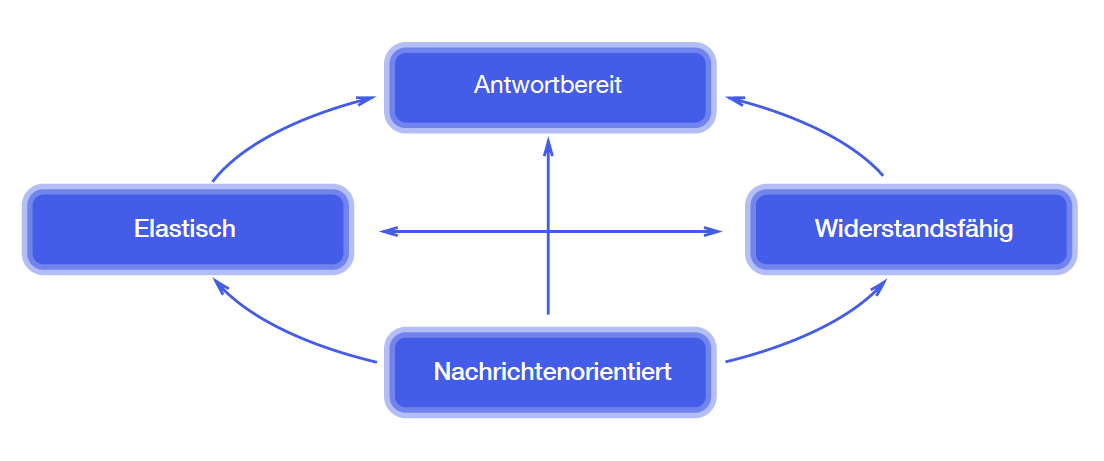
\includegraphics[width=1\textwidth]{Abb/manifest4achsen.PNG}
	\caption{Die vier relevanten Bestandteile für ein reaktives System.Quelle \cite{Boner.2014}}
	\label{pic:manifest4}
\end{figure}
\begin{itemize}
	\item \textbf{Antwortbereit (engl. responsive):}\\ Ein System muss immer zeitgerecht antworten. Die Antwortbereitschaft ist die Grundlage für die Benutzbarkeit besagten Systems. Ebenso wird um eine Fehlerbehandlung durchführen zu können eine geregelte Antwortbereitschaft vorausgesetzt.
	\item \textbf{Widerstandsfähig (engl. resilient):}\\ Ein System muss auch bei Ausfällen die Antwortbereitschaft aufrecht erhalten. Dies wird durch Replikation der Funktionalität, der Isolation von Komponenten sowie dem Delegieren von Verantwortlichkeiten erzielt. 
	\item \textbf{Elastisch (engl. elastic):}\\ Das System muss bei sich ändernden Lasten die Funktionalität und Antwortbereitschaft aufrecht erhalten. Ressourcen müssen den auftretenden Lasten, ob steigend oder sinkend, angepasst werden können. Ebenso müssen Engpässe innerhalb des Systems unterbunden werden um die Elastizität zu bewahren.
	\item \textbf{Nachrichtenorientiert (engl. message driven):}\\ Ein loses System soll zur Kommunikation zwischen den Komponenten auf asynchrone, ortsunabhängige Nachrichtenübermittlung zurück greifen. Somit ist nicht relevant auf welchen Rechner die einzelnen Komponenten ausgeführt werden, wodurch wiederum eine gute Skalierbarkeit erreicht werden kann.
\end{itemize}
Das Manifest beschreibt jedoch nicht den Zusammenhang von Reactive Systems zum Reactive Programming. Wohl aus diesem Grund hat Jonas Bonér einen weiteren Artikel verfasst, der sich dieser Thematik annimmt \cite{Boner.}. Die grundlegenden Unterschiede wurde in dem Artikel wie folgt zusammengefasst:
\begin{itemize}
	\item Reactive Programming ist eine Teilmenge von reaktiven Systemen auf Implementierungsebene
	\item Reactive Programming liefert Leistung und effektive Ressourcennutzung auf Komponentenebene, speziell für Softwareentwickler.
	\item Reaktive Systeme hingegen bieten Robustheit und Elastizität auf Systemebene zur Gestaltung von Cloud-kompatiblen oder verteilten Anwendungen, speziell für Softwarearchitekten oder DevOps, also der Möglichkeit eine schnelle und qualitativ hochwertige Software zu entwickeln und auszurollen.
	\item Es ist von großem Vorteil Reactive Programming innerhalb der Bestandteile von reaktiven Systemen zu verwenden.
	\item Es is ebenso von Vorteil reaktive Systeme zur Interaktion zwischen reaktiv programmierten Komponenten zu verwenden.
\end{itemize}
Wie aus diesen Punkten klar wird, liegt also der genaue Unterschied zwischen Reactive Programming und Reactive Systems darin, aus welcher Perspektive die Betrachtung stattfindet. Architektonisch wird von Systemen gesprochen, die innerhalb und zur Interaktion mit anderen reaktiv reagiert. Betrachtet man das Ganze aus Entwicklersicht in Bezug auf eine Komponente, kann diese unter Zuhilfenahme von Reactive Programming für ein asynchrones, paralleles Verhalten entwickelt werden. Wie Jonas Bonér schon schreibt, ist das Zusammenspiel beider sehr oft hilfreich um das gewünschte Ziel zu erreichen. Ein weiterer wichtiger Punkt ist die Unterscheidung von \textit{ereignisorientiert} zu \textit{nachrichtenorientiert}. Nachrichten werden auf Systemebene genutzt. im Gegensatz zu Ereignissen sind Nachrichten klar an einen Empfänger adressiert. Ereignisse treten auf und müssen beobachtet werden um das gewünschte Resultat zu erzielen. Nachrichten sind somit gut geeignet bekannte Empfänger in einem verteilten System, zum Beispiel über das Netzwerk, zu kontaktieren. Innerhalb der Komponente besteht die Funktion (man denke hier wieder an die Benutzeroberfläche) oft aus der Reaktion auf Ereignisse unterschiedlicher Art die direkt in der Komponente verarbeitet werden sollen. Somit herrscht hier ein ereignisgetriebenes Verhalten. 

\section{Abgrenzung Reactive Programming von Functional Reactive Programming}
Auf der Suche nach einer Definition zu Reactive Programming stößt man oft auf den Begriff Functional Reactive Programming. Teilweise werden die Begriffe sogar synonym verwendet \cite{Nurkiewicz.2017}. Grundlegend betrachtet man bei den bekannten Programmierparadigmen zwischen imperativen und deklarativen Paradigmen, wobei zum Beispiel die objektorientierte Programmierung im imperativen und funktionale Programmierung im deklarativen Bereich angesiedelt wird. Funktionale Programmierung zeichnet vor allem die Nutzung des Lambda-Kalküls aus \cite{lamdakalk}. Ein Lambda-Ausdruck wird in der Mathematik wie folgt dargestellt:
\begin{displaymath}
\lambda x.x+2
\end{displaymath}
Dieser Ausdruck besagt, dass jeder Wert $x$ auf $x+2$ abgebildet wird.
Statt Rechenanweisungen werden Programme als Menge von Definitionen beschrieben, die mathematisch eine Abbildung von Eingabedaten auf Ausgabedaten darstellt und gleichzeitig selbst aus Funktionsaufrufen zusammengesetzt sind \cite{fpwiki}. Wird eine funktionale Programmiersprache nun um den Faktor Zeit erweitert kann ein reaktives Verhalten erreicht werden. Diese Art der Realisierung nennt man Functional Reactive Programming \cite{hsklwiki}. Dieser Zeitfaktor zeigt sich im Funktionalen in der kontinuierlichen Wertänderung im Laufe der Zeit. Die Verwechslung der Begriffe entsteht wenn man sich zum Beispiel Java 8 anschaut. Mit Java 8 nahm die Klasse der Funktionen sowie die Lambda-Ausdrücke Einzug in die objektorientierte Programmiersprache Java. In Java-Code werden Lambda-Ausdrücke wie folgt dargestellt:
\begin{lstlisting}[language=java, caption={Lambda Beispiel in Java}, float=hbt, label=lst:LambdaJava, frame=single]
List< Integer > list = Arrays.asList( 1, 2, 3, 4, 5 );
list.forEach( element -> System.out.println( "Number" + element ) );
\end{lstlisting}
In Listing \ref{lst:LambdaJava} wird jedes der Listenelemente auf die Konsolenasugabe mit konkateniertem String abgebildet. Dadurch wird ein ähnliches Verhalten der funktionalen Programmierung reproduziert. Somit sind funktionale Eigenschaften zwar in Java vorhanden, trotzdem kann Java nicht als funktionale Programmiersprache verstanden werden. Wird auch hier nun der Faktor Zeit mit betrachtet, kann darin der essentielle Unterschied ausgemacht werden. Wird beim Functional Reactive Programming von einer Wertänderung im Laufe der Zeit gesprochen, ist beim Reactive Programming von konkreten Werten zu sprechen die im Laufe der Zeit ausgegeben werden. Also findet keine Änderung des Wertes statt, es werden neue Werte über einen Zeitraum weiter gereicht. 